%
% GNU courseware, Zhang Jiadong, 2018
%

\section{差分进化}\fontsize{12pt}{12pt}\selectfont

\subsection{定义}
\begin{frame}{定义}
	{\bf差分进化}是一种基于群体智能的全局优化方法,其主要通过种群内个体之间的协同合作
		和相互竞争来产生群体智能,进一步指导进化过程的全局搜索。
\end{frame}

\subsection{算法思想}
\begin{frame}{算法思想}
	\begin{figure}
		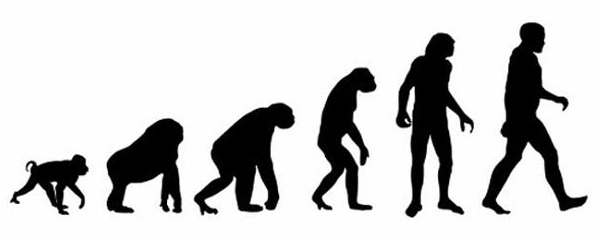
\includegraphics [width =1.0\textwidth]{../images/evolution.png}
	\end{figure}
	通过种群之间的\textbf{个体差异}和\textbf{优胜劣汰}的竞争策略产生新的个体,最终使种群接近或达到全局最优解。
\end{frame}

\subsection{算法框架}
\begin{frame}{算法框架}\small
	\begin{figure}
		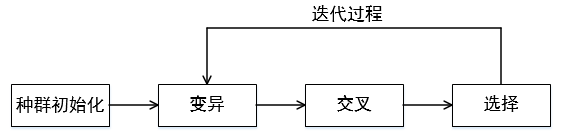
\includegraphics [width =1.0\textwidth]{../images/framework.png}
		\vspace{-1.2cm}
	\end{figure}
	\begin{itemize}
		\item {\bf 种群初始化}在解空间中随机、均匀地产生$M$个个体,每个个体由$n$个染色体组成,作为第$0$代种群,标记为
		\begin{equation*}
			\begin{split}
				X_i(0)=&\left(x_{i,1}(0),x_{i,2}(0),\cdots,x_{i,n}(0)\right)\\
				& i=1,2,\cdots,M
			\end{split}
		\end{equation*}
		\item {\bf 变异、交叉、选择 }三步操作迭代执行,直到算法收敛。第$g$次迭代的第$i$个个体标记为
		\begin{equation*}
			\begin{split}
				X_i(g)=&\left(x_{i,1}(g),x_{i,2}(g),\cdots,x_{i,n}(g)\right)\\
				& i=1,2,\cdots,M
			\end{split}
		\end{equation*}
	\end{itemize}
\end{frame}

\begin{frame}{种群初始化}
	在$n$维空间里随机产生满足约束条件的$M$个染色体,第$i$个染色体的第$j$个维取值方式如下(rand(0,1)产生0到1的均匀分布的随机数) :
	\begin{equation*}
		\begin{split}
			x_{i,j}(0) &= L_j + rand(0,1)\left(U_j-L_j\right)\\
			& i = 1,2,\cdots,M\\
			& j = 1,2,\cdots,n\\
		\end{split}
	\end{equation*}
\end{frame}

\begin{frame}{变异算子}
	在第$g$次迭代中,对个体$X_i(g)=\left(x_{i,1}(g),x_{i,2}(g),\cdots,x_{i,n}(g)\right)$,从种群中随机选择$3$个个体 $X_{p1}(g),X_{p2}(g),X_{p3}(g)$,且$ p1 \neq p2 \neq p3\neq i$, 则
	$$H_{i}(g) = X_{p1}(g)+ F\cdot\left(X_{p2}(g)-X_{p3}(g)\right)$$
	% 其中$\Delta_{p2,p3}(g)=X_{p2}(g)-X_{p3}(g)$是差分向量;$F$是缩放因子,用于控制差分向量的影响力.
	\begin{figure}
		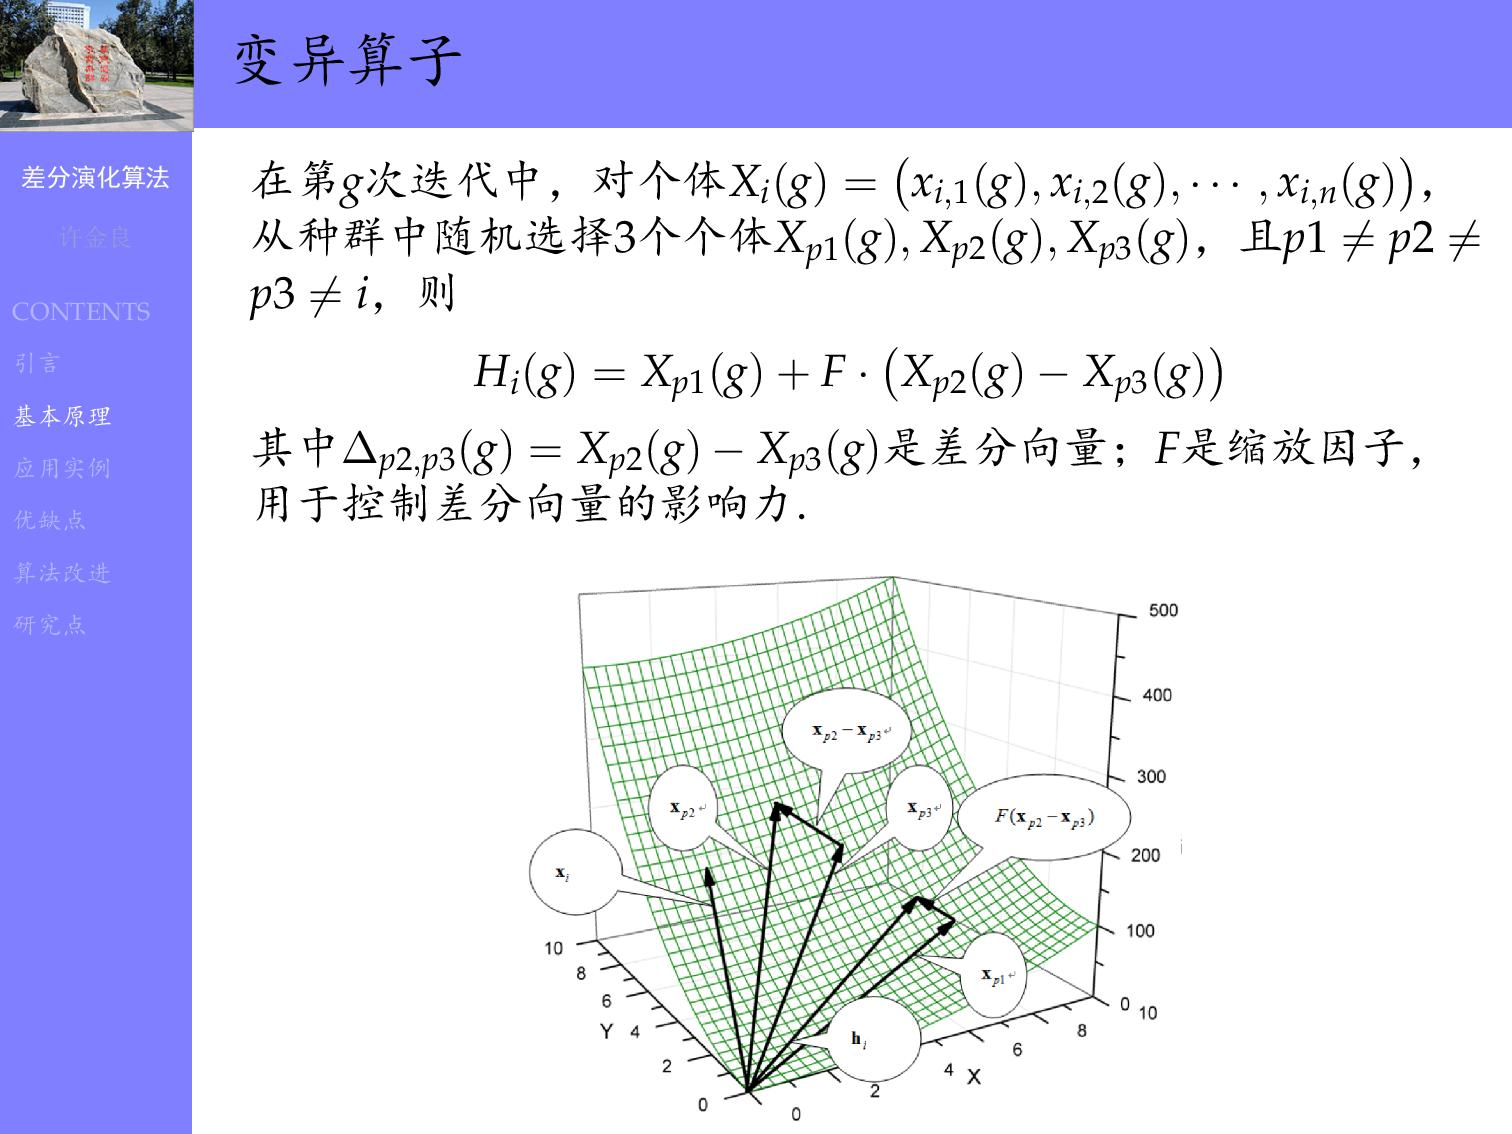
\includegraphics [width =0.55\textwidth]{../images/mutation.png}
	\end{figure}
\end{frame}

\begin{frame}{交叉算子}
	交叉操作可以增加种群的多样性,方法如下:
	$$
	v_{i,j}(g)=
	\begin{cases}
	h_{i,j}(g), rand(0,1)\le cr\\
	x_{i,j}(g), else
	\end{cases}
	$$
	其中$cr\in[0,1]$为交叉概率,$rand(0,1)$是$[0,1]$上服从均匀分布的随机数。

	\begin{figure}
		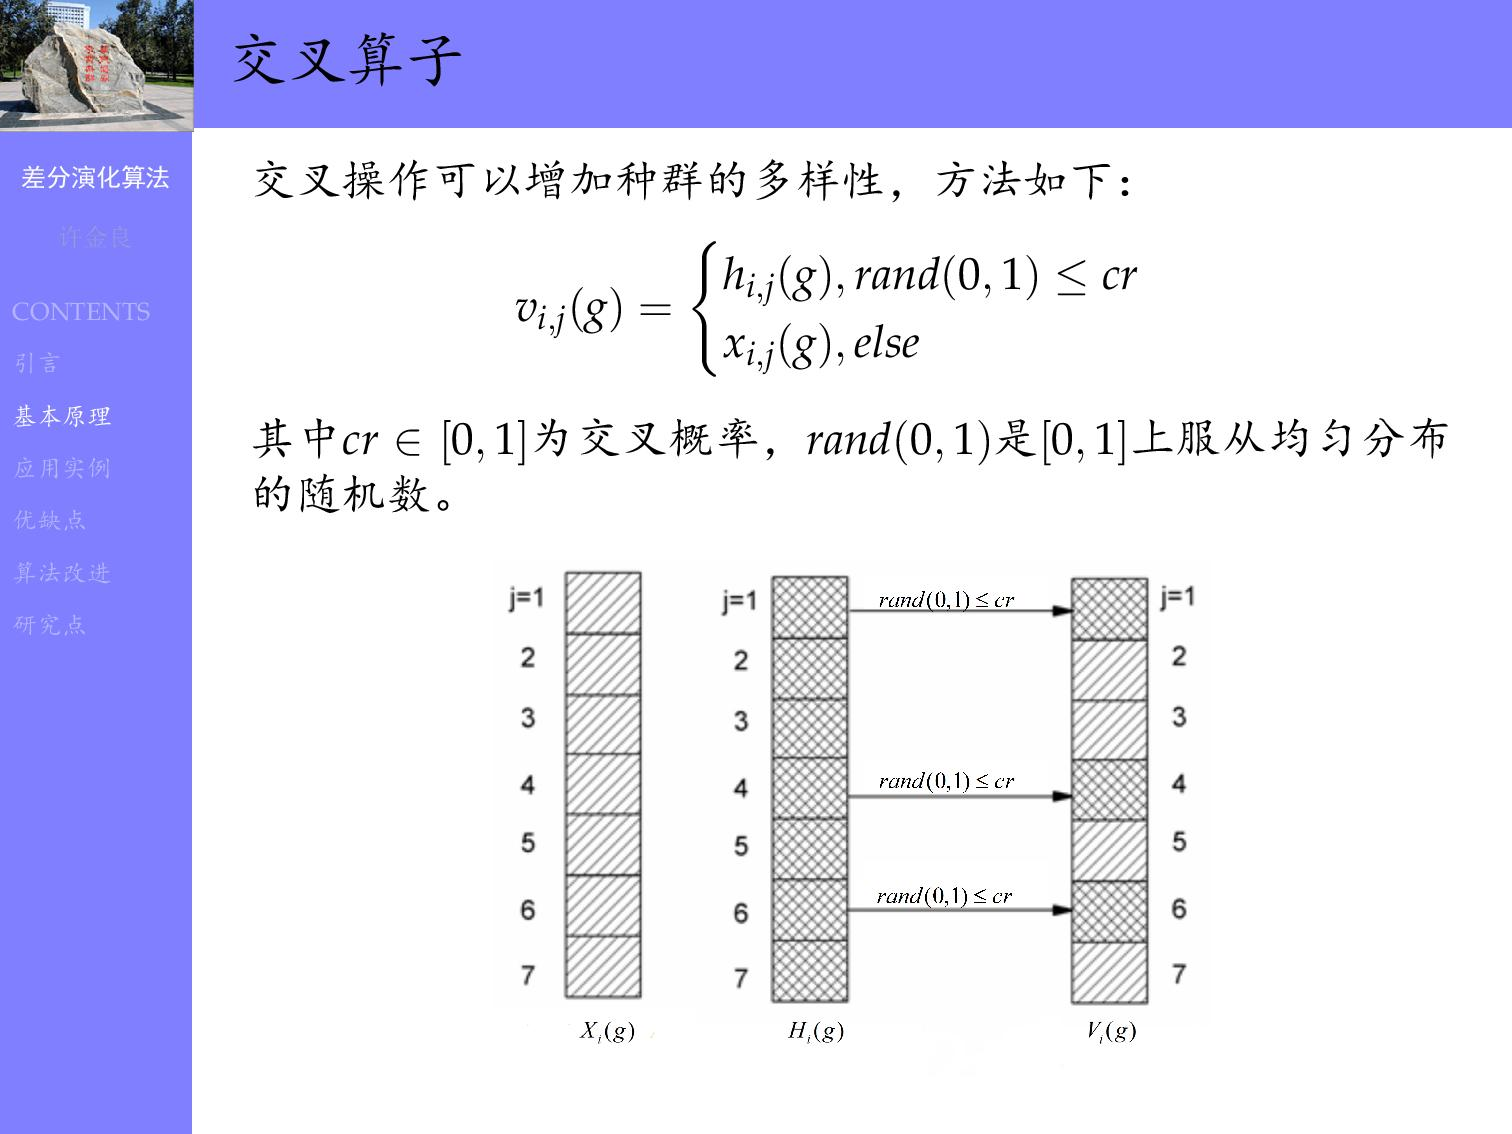
\includegraphics [width =0.55\textwidth]{../images/cross.png}
	\end{figure}
\end{frame}

\begin{frame}{选择算子}
首先查看根据评价函数选择$V_i(g)$ 或 $X_i(g)$ 作为$X_i(g+1)$
$$
	X_i(g+1) =
	\begin{cases}
	V_i(g),\qquad \mathrm{if} \quad f(V_i(g))< f(X_i(g))\\
	X_i(g),\qquad else
	\end{cases}
$$

可以看出:
	\begin{itemize}
		\item 对每个个体,$X_i(g+1)$要好于或持平$X_i(g)$。
		\item 肯定会收敛于最优点(可能是局部最优)。
		\item {\bf 变异、交叉} 操作有助于突破局部最优到达全局最优。
	\end{itemize}
\end{frame}

\subsection{应用实例}
\begin{frame}{差分进化算法寻找函数最优解}
	定义关于参数$x, y$的函数表达式如下:
	$$f(x,y)=-20e^{-0.2\sqrt{\frac{x^2+y^2}{2}}}-e^{\frac{\cos2\pi x+\cos2\pi y}{2}}+20+e$$
	求函数的最小值。
	\begin{itemize}
		\item 个体定义:$P$, $P[0]$表示$x$, $P[1]$表示$y$。
		\item 取值范围:$-5 < x, y < 5$。
		\item 适应度定义:$f(x,y)$。
	\end{itemize}
\end{frame}

\begin{frame}{差分进化算法寻找函数最优解}
	用差分进化算法求解,效果如右图所示(参数设置:$N=20, F=0.5, cr=0.5$,迭代次数 $T=300$)
	\begin{columns}
		\begin{column}{0.45\textwidth}
			\begin{figure}
				\vspace{-0.8cm}
				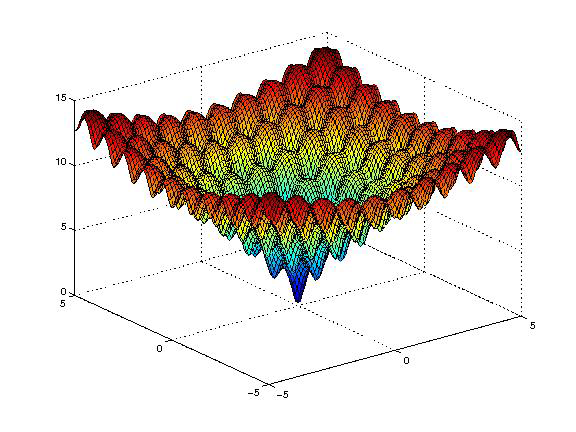
\includegraphics [width =2.0in]{../images/function.png}
			\end{figure}
		\end{column}
		\begin{column}{0.55\textwidth}
			\begin{figure}
				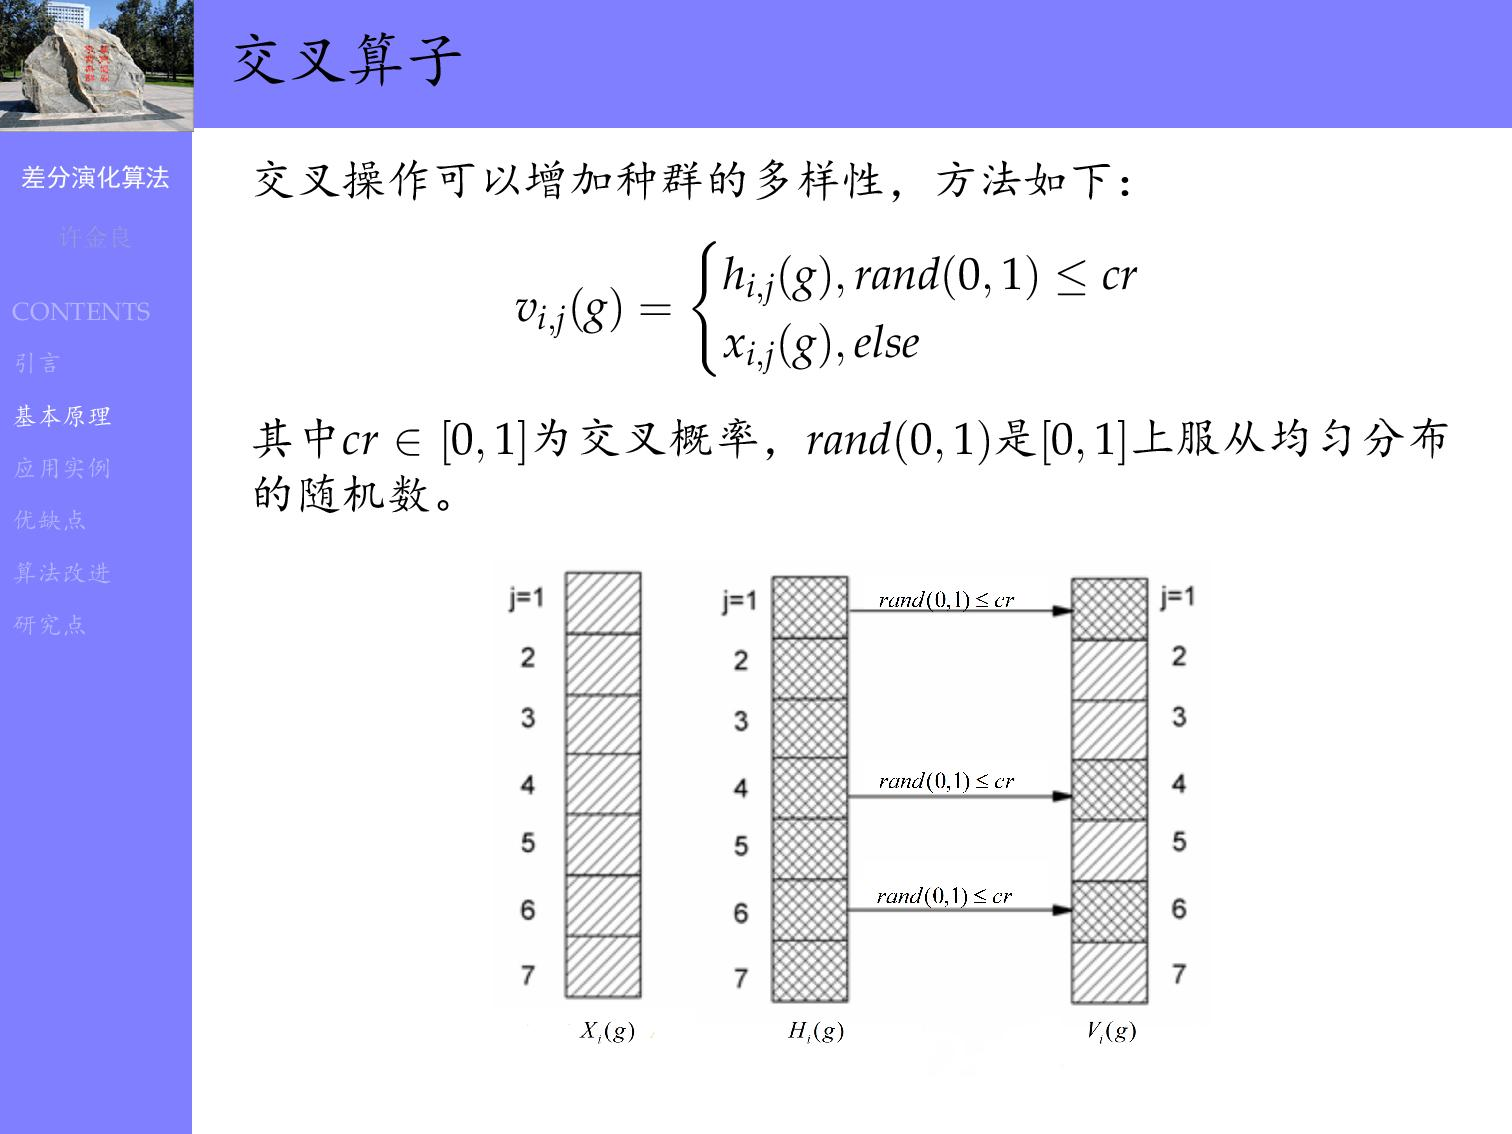
\includegraphics [width =2.0in]{../images/curve.png}
			\end{figure}
		\end{column}
	\end{columns}
\end{frame}

\subsection{优缺点}
\begin{frame}{优缺点}
和其他进化算法相比,差分进化算法具有以下优点:
	\begin{enumerate}
		\item 在非凸、多峰、非线性、连续不可微函数优化问题上表现出极强的稳健性。
		\item 收敛速度快。
		\item 操作简单,容易实现。
	\end{enumerate}
	缺点:
	\begin{enumerate}
		\item 算法后期个体间差异逐渐缩小,收敛速度慢,容易陷入局部最优。
		\item 控制参数和学习策略对算法性能有着重要的影响,并且高度依赖于优化问题的本质。
		\item 有时需要过多的迭代才能搜索到全局最优。
	\end{enumerate}
\end{frame}


\subsection{算法改进}
\subsubsection{参数控制}

\begin{frame}{参数的选取}
%参数选择主要涉及群体规模$M$,缩放因子$F$,以及交叉概率$cr$的设定\footnote{
%各研究人员得到的经验参数值往往不一致,甚至相互矛盾,所以要具体问题具体分析。}
	\begin{itemize}
		\item $M$:一般介于$5\times n$与$10\times n$之间,但不能少于$4$,否则变异算子无法进行;
		\item $F$:一般在$[0,2]$之间选择,通常取$0.5$;
		\item $cr$:一般在$[0,1]$之间选择,比较好的选择应在$0.3$左右。$cr$取值偏大,收敛速度会加快,但易发生早熟现象。
	\end{itemize}
\end{frame}

\begin{frame}{参数的自适应调整($F$)}
	将变异算子中随机选择的三个个体进行从优到劣的排序,得到$X_b,X_m,X_w$,对应适应度$f_b,f_m,f_w$,则变异算子改为:
	$$V_i=X_b+F_i\left(X_m-X_w\right)$$
	同时,$F$的取值根据生成差分向量的两个个体自适应变化,平衡全局搜索和局部搜索之间的矛盾。
	$$F_i = F_l +\left(F_u-F_l\right)\frac{f_m-f_b}{f_w-f_b}$$
	其中,$$F_l=0.1,F_u=0.9$$
\end{frame}

\begin{frame}{参数的自适应调整($cr$)}
	对于适应度好的解,取较小的$cr$,使得该解进入下一代的机会增大;
	对于适应度差的解,则取交大的$cr$,加快改变该个体的结构,使该解被淘汰掉。
	$$
	cr_i =
	\begin{cases}
		cr_l+\left(cr_u-cr_l\right)\frac{f_i-f_{min}}{f_{max}-f_{min}}  \qquad \mathrm{if} \quad f_i>\bar{f} \\
		cr_l \qquad\qquad \qquad \qquad \qquad \quad \mathrm{if}\quad f_i<\bar{f}
	\end{cases}
	$$
	其中 $f_i$是个体$X_i$的适应度,$f_{min}$和$f_{max}$分别是当前种群中最差和最优个体的适应度,
	$\bar{f}$是当前种群适应度平均值,$cr_l$和$cr_u$分别是$cr$的下限和上限,一般$cr_l=0.1,cr_u=0.6$。
\end{frame}

\subsubsection{变异策略}
\begin{frame}{变异策略}
	变异策略表示为$DE/a/b$,其中$a$表明被变异个体的选择方式,$b$表明差向量的个数。
		\begin{enumerate}
		\item {\bf DE/rand/1:}\\\qquad$V_i = X_{p1}+F\left(X_{p2}-X_{p3}\right)$
		\item {\bf DE/best/1:}\\\qquad$V_i = X_{best}+F\left(X_{p1}-X_{p2}\right)$
		\item {\bf DE/current to best/1:}\\\qquad$V_i = X_{i}+F\left(X_{best}-X_{i}\right)+F\left(X_{p1}-X_{p2}\right)$
		\item {\bf DE/best/2:}\\\qquad$V_i=X_{best}+F\left(X_{p1}-X_{p2}\right)+F\left(X_{p3}-X_{p4}\right)$
		\item {\bf DE/rand/2:}\\\qquad$V_i = X_{p1}+F\left(X_{p2}-X_{p3}\right)+F\left(X_{p4}-X_{p5}\right)$
	\end{enumerate}
\end{frame}

% \end{CJK*}
% \end{document}